\documentclass[ignorenonframetext,]{beamer}
\usetheme{Warsaw}
\usepackage{amssymb,amsmath}
\usepackage{ifxetex,ifluatex}
\usepackage{fixltx2e} % provides \textsubscript
\ifxetex
  \usepackage{fontspec,xltxtra,xunicode}
  \defaultfontfeatures{Mapping=tex-text,Scale=MatchLowercase}
\else
  \ifluatex
    \usepackage{fontspec}
    \defaultfontfeatures{Mapping=tex-text,Scale=MatchLowercase}
  \else
    \usepackage[utf8]{inputenc}
  \fi
\fi

% Comment these out if you don't want a slide with just the
% part/section/subsection/subsubsection title:
\AtBeginPart{
  \let\insertpartnumber\relax
  \let\partname\relax
  \frame{\partpage}
}
\AtBeginSection{
  \let\insertsectionnumber\relax
  \let\sectionname\relax
  \frame{\sectionpage}
}
\AtBeginSubsection{
  \let\insertsubsectionnumber\relax
  \let\subsectionname\relax
  \frame{\subsectionpage}
}

\setlength{\parindent}{0pt}
\setlength{\parskip}{6pt plus 2pt minus 1pt}
\setlength{\emergencystretch}{3em}  % prevent overfull lines
\setcounter{secnumdepth}{0}

\title{Python Web Development}
\author{Antoine Pietri \& Paul Hervot}
\date{2013-12-06}

\usepackage{minted}\begin{document}
\frame{\titlepage}

\section{Introduction}\label{introduction}

\begin{frame}[fragile]{Python Web Development}

\begin{center}
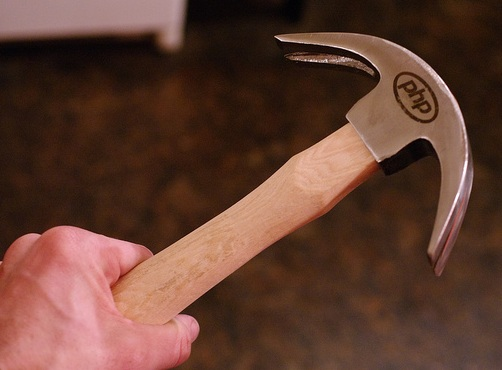
\includegraphics[width=9cm]{img/php}
\end{center}

\end{frame}

\begin{frame}[fragile]{Introduction}

\begin{itemize}[<+->]
\itemsep1pt\parskip0pt\parsep0pt
\item
  This is not a tutorial
\item
  There are plenty frameworks and a lot of documentation everywhere on
  the Internet
\item
  More like a global current overview to help someone new to Python
  Development
\end{itemize}

\end{frame}

\section{Getting started}\label{getting-started}

\begin{frame}[fragile]{Python}

\begin{itemize}[<+->]
\itemsep1pt\parskip0pt\parsep0pt
\item
  You will need Python.
\item
  Which version to choose is a very difficult choice.
\item
  Python 3: the future, but made some backwards incompatible changes
\item
  Be sure everything you want to use supports it
\item
  Python 2 is generally the poor but reasonable choice :(
\end{itemize}

\end{frame}

\begin{frame}[fragile]{pip}

\begin{itemize}[<+->]
\itemsep1pt\parskip0pt\parsep0pt
\item
  For installing Python librairies, use pip
\item
  Package manager for Python libs
\item
  Very handy
\item
  You will use it often to install modules, especially with Django
\end{itemize}

\end{frame}

\begin{frame}[fragile]{virtualenv}

\begin{itemize}[<+->]
\itemsep1pt\parskip0pt\parsep0pt
\item
  You can install modules in your user home or globally, but that's
  dirty
\item
  virtualenv is the solution!
\item
  Keep the same environment with the versions of libraries you want
\end{itemize}

\end{frame}

\begin{frame}[fragile]{VCS}

\begin{itemize}[<+->]
\itemsep1pt\parskip0pt\parsep0pt
\item
  You're of course \emph{planning} to use version control, right?
\item
  Anything is better than nothing
\end{itemize}

\end{frame}

\section{Framework}\label{framework}

\begin{frame}[fragile]{Connect your code to a browser}

\begin{itemize}[<+->]
\itemsep1pt\parskip0pt\parsep0pt
\item
  This is not PHP
\item
  You can't just drop some files in a folder and tell apache to use them
\item
  That's really a \emph{bad} approach anyway
\item
  You should use a \textbf{web framework} that will do a lot of job for
  you
\end{itemize}

\end{frame}

\begin{frame}[fragile]{Workflow}

\begin{itemize}[<+->]
\itemsep1pt\parskip0pt\parsep0pt
\item
  Install it
\item
  Generate the boilerplate
\item
  Configure the necessary
\item
  Start a development server
\item
  Code!
\end{itemize}

\end{frame}

\begin{frame}[fragile]{Flask}

\begin{itemize}[<+->]
\itemsep1pt\parskip0pt\parsep0pt
\item
  Simple
\item
  Extensible
\item
  No boilerplate, works ``out of the box''
\end{itemize}

\end{frame}

\begin{frame}[fragile]{Flask example}

\begin{minted}{python}

    from flask import Flask
    app = Flask(__name__)

    @app.route("/")
    def hello():
        return "Hello World!"

        if __name__ == "__main__":
            app.run()

\end{minted}

\end{frame}

\end{document}
